\section{Results}
\label{sec:results}

\begin{table}[t]
\centering
\caption{Closed-book accuracy on the 125-question layered audit set (3-shot
completion, greedy decoding; letters for multiple choice, exact match after
normalization otherwise). ``Quizzed-facts aug.''\ is the ablation whose
augmentation covered only the 461 pilot-quizzed facts.}
\label{tab:subset}
\small
\setlength{\tabcolsep}{3.2pt}
\begin{tabular}{lcccccc}
\toprule
Model & Total & L1$_{40}$ & L2$_{26}$ & L3$_{32}$ & L4$_{20}$ & L5$_{7}$ \\
\midrule
Qwen3.5-9B-Base       & 43.2\% & 7  & 4  & 29 & 11 & 3 \\
\; + quizzed-facts aug. & 55.2\% & 20 & 4  & 31 & 9  & 5 \\
Claude Opus 5         & 72.0\% & 23 & 18 & 32 & 11 & 6 \\
\textbf{DAPT (ours)}  & \textbf{92.8\%} & \textbf{40} & \textbf{19} & \textbf{32} & \textbf{20} & 5 \\
\bottomrule
\end{tabular}
\end{table}

\begin{table}[t]
\centering
\caption{Full bank: all 1{,}776 auto-generated questions, of which 1{,}651
were never inspected during development.}
\label{tab:fullbank}
\small
\setlength{\tabcolsep}{2.6pt}
\begin{tabular}{lcccccc}
\toprule
Model & Total & L1$_{419}$ & L2$_{53}$ & L3$_{53}$ & L4$_{25}$ & L5$_{1226}$ \\
\midrule
Qwen3.5-9B-Base      & 41.2\% & 7\%  & 32\% & 89\% & 52\% & 51\% \\
Claude Opus 5        & 72.2\% & 28\% & 79\% & 98\% & 52\% & 86\% \\
\textbf{DAPT (ours)} & \textbf{81.6\%} & \textbf{97\%} & 68\% & \textbf{100\%} & \textbf{100\%} & 76\% \\
\bottomrule
\end{tabular}
\end{table}

\paragraph{Audit set.} Table~\ref{tab:subset} and Figure~\ref{fig:ladder}:
the full recipe reaches 92.8\%, +20.8 points over Claude Opus~5 and +49.6 over
its own base. The quizzed-facts ablation row is the coverage result of
\S\ref{sec:d4} in tabular form: +13 questions on covered layers, base-level
everywhere else.

\paragraph{Anti-overfitting check.} Because the audit set is the only part of
the benchmark we ever looked at while iterating, the full bank
(Table~\ref{tab:fullbank}) is the honest test: on the 379 never-inspected L1
fact questions the model scores 97\%, matching its 100\% on the inspected 40.
The subset number is not sample luck, and the augmentation's full-coverage
property is real.

\paragraph{Complementary failure profiles.} Figure~\ref{fig:layers} shows why
``beats Opus'' is the right summary but not the interesting one. The frontier
model wins wherever semantic association helps: issue-title$\rightarrow$
repository attribution (86\%), memory-region ownership (26/27), documentation
semantics (98\%). It collapses on pure memorization: 18\% on register offsets.
The adapted 9B is the mirror image---97\% on offsets, 100\% on
driver--register links, weaker on numeric range reasoning (region ownership
11/27). Knowledge injection buys exactly the layer that retrieval-free
internal assistance needs and that scale alone does not provide.

\paragraph{Compute.} Every training run in this study is a single
4$\times$H100 node for 77 minutes; evaluation of the full bank is one
GPU-hour under vLLM.

\begin{figure}[t]
  \centering
  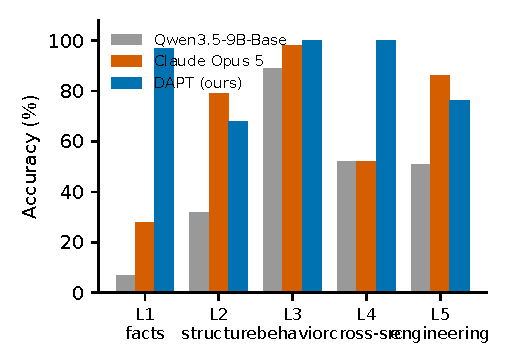
\includegraphics[width=\linewidth]{figures/fig2_layers.pdf}
  \caption{\textbf{Layer profiles on the full 1{,}776-question bank.} The
  frontier model and the adapted 9B fail in opposite places: Opus~5 wins on
  association-friendly layers (L3, L5) but scores 28\% on L1 facts; the
  DAPT model holds 97--100\% on facts and cross-source links. L2 mixes
  memorizable items (sizes, pins) with numeric range reasoning, where the
  adapted model remains weak.}
  \label{fig:layers}
\end{figure}
